\chapter{Strings}


% \kactlimport{Hashing.h}
\kactlimport{KMP.h}
\kactlimport{Zfunc.h}
\kactlimport{Manacher.h}
\kactlimport{MinRotation.h}

% \begin{lecture}{AC自动机}
% 	$\texttt{Aho-Corasick}$自动机用于$\texttt{多模式串匹配}$

% 	给定若干模式串：
% 	\[
% 	\begin{cases}
% 		\texttt{he}\\
% 		\texttt{she}\\
% 		\texttt{his}\\
% 		\texttt{hers}
% 	\end{cases}
% 	\]
	
% 	再给一个文本串:$\texttt{ushers}$

% 	要找出每个模式串在哪些位置出现。
% 	朴素做法是每个模式串跑一次KMP,
% 	总复杂度约为:$O(\text{模式串个数}\times\text{文本长度})$

% 	AC自动机的目标:
% 	\begin{itemize}[label={}]
% 		\item 构建:$O(\text{所有模式串总长}\times\text{字符集大小})$
% 		\item \text{find}:$O(\text{文本长度}+\text{匹配输出量})$
% 		\item \text{findAll}:$\text{最坏达}O(\text{文本长度}\times\text{模式串数})$
% 	\end{itemize}
	
	
% 	\begin{flalign*}
% 	\text{直接输出链} &: \texttt{end} \to \cdots \to \texttt{start},\\
% 	\text{fail 输出链} &: \texttt{N[y].end} \to \cdots,\\
% 	\text{拼接后} &: \texttt{end} \to \cdots \to \texttt{start}
% 		\to \texttt{N[y].end} \to \cdots.&
% 	\end{flalign*}
	
% \end{lecture}
% \kactlimport{AhoCorasick.h}

% \begin{lecture}{后缀数组}
% 	\textbf{定义.} 将字符串的所有后缀按字典序排序,
% 	只保存后缀起点:
% 	\[
% 		\texttt{sa[i]}=\text{字典序第} i \text{小的后缀起点}.
% 	\]
% 	若 $\texttt{s=banana}$, 排序后为
% 	\[
% 	\texttt{a},\texttt{ana},\texttt{anana},\texttt{banana},
% 	\texttt{na},\texttt{nana},
% 	\]
% 	因此$\texttt{sa}=[5,3,1,0,4,2]$。
% 	反数组通常记为 $\texttt{rk}$:
% 	\[
% 		\texttt{rk[pos]}=\text{后缀}\texttt{s[pos...]}\text{的排名}.
% 	\]
% 	本板子构造结束后用 $\texttt{x[i]}$ 承担 $\texttt{rk[i]}$ 的角色。

% 	\textbf{哨兵.} 在\texttt{s}后加入严格小于所有字符的哨兵。
% 	本板子使用
% 	\[
% 		\texttt{s.push\_back(0)}
% 	\]
% 	故输入不能包含 $\texttt{nul}$ 字符。若原串长为 $n$,
% 	则哨兵所在的空后缀最小:
% 	\[
% 		\texttt{sa[0]}=n.
% 	\]
% 	所以返回数组大小为 $n+1$, 处理原串后缀时常从
% 	$\texttt{sa[1]}$ 开始看。

% 	\textbf{循环位移到后缀数组.} cp-algorithms 的构造本质上先排序
% 	\textbf{循环位移}而非直接排序后缀。循环位移把字符串看成首尾相接,
% 	位置 $i$ 开始的循环串为
% 	\[
% 		\texttt{s[i...] + s[0...i-1]}.
% 	\]
% 	更一般地, 当区间右端绕回开头时:
% 	\[
% 		\texttt{s[i..j]}
% 		=
% 		\texttt{s[i..n-1] + s[0..j]}
% 		\qquad (\texttt{i>j}),
% 	\]
% 	下标按模 $n$ 理解。

% 	排序循环位移如何变成排序后缀? 在原串后加入最小哨兵后,
% 	任何真实后缀都可看作一个循环位移中哨兵之前的前缀。由于哨兵
% 	严格小于所有普通字符, 两个后缀第一次分出长短时, 较短者会先遇到哨兵,
% 	字典序也正好更小。因此
% 	\[
% 		\text{sort cyclic shifts of }(s+\text{'0'})
% 		\Longleftrightarrow
% 		\text{sort suffixes of }s,
% 	\]
% 	只不过结果最前面多出哨兵位置对应的空后缀。本板子不删除它,
% 	所以保留 $\texttt{sa[0]}=n$。

% 	例如 $\texttt{dabbb\$}$ 的循环位移排序中, 去掉哨兵后的前缀顺序为
% 	\[
% 		\texttt{abbb},\texttt{b},\texttt{bb},\texttt{bbb},\texttt{dabbb},
% 	\]
% 	这正是 $\texttt{dabbb}$ 的后缀字典序。

% 	\textbf{倍增思想.} 已知每个位置开始、长度为 $j$ 的子串排名后,
% 	长度为 $2j$ 的子串可由二元组表示:
% 	\[
% 		\bigl(\texttt{rank[i]},\texttt{rank[i+j]}\bigr).
% 	\]
% 	本板子中
% 	\[
% 		\texttt{sa}=p,\qquad
% 		\texttt{x}=c,\qquad
% 		\texttt{y}=\text{临时起点/旧排名},\qquad
% 		\texttt{ws}=\text{计数桶},
% 	\]
% 	其中 $p,c$ 对应 cp-algorithms 中的有序位置数组与等价类数组。
% 	主循环
% 	\[
% 		\texttt{j}=0,1,2,4,8,\ldots
% 	\]
% 	每轮把已知长度翻倍。第一次 $\texttt{j=0}$ 可视为按单字符排序,
% 	因为初始化时已有 $\texttt{x[i]=s[i]}$。

% 	\begin{center}
% 		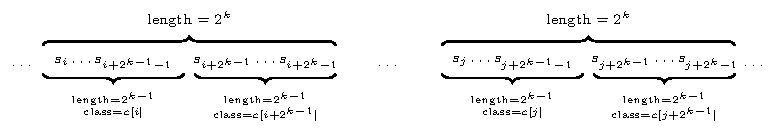
\includegraphics[width=\linewidth]{content/strings/SuffixArrayCyclicPairs.pdf}
% 	\end{center}

% 	\textbf{基数排序.} 每轮需要按
% 	\[
% 		\bigl(\texttt{x[i]},\texttt{x[i+j]}\bigr)
% 	\]
% 	排序。直接比较二元组会多一个 $\log n$, 因此使用计数排序。
% 	代码先构造 $\texttt{y}$, 使其已按第二关键字有序;
% 	再稳定地按第一关键字 $\texttt{x[y[i]]}$ 计数排序:
% 	\[
% 		\texttt{sa[--ws[x[y[i]]]]=y[i]}.
% 	\]
% 	于是每轮为 $O(n)$, 轮数为 $O(\log n)$, 总复杂度
% 	\[
% 		O(n\log n).
% 	\]

% 	\textbf{重编号.} 排序完成后, 相邻后缀 $\texttt{a=sa[i-1]}$,
% 	$\texttt{b=sa[i]}$ 的新排名由旧二元组决定:
% 	\[
% 		(\texttt{old[a]},\texttt{old[a+j]})
% 		=
% 		(\texttt{old[b]},\texttt{old[b+j]})
% 		\Rightarrow
% 		\texttt{new[a]}=\texttt{new[b]}.
% 	\]
% 	对应代码为
% 	\[
% 		\texttt{(y[a] == y[b] \&\& y[a+j] == y[b+j])}.
% 	\]
% 	若不同排名数 $\texttt{p}$ 已达到 $\texttt{n}$, 所有后缀排名唯一,
% 	构造结束。

% 	\textbf{LCP/height.} 后缀数组常配合相邻最长公共前缀数组:
% 	\[
% 		\texttt{lcp[i]}
% 		=
% 		\operatorname{LCP}
% 		\bigl(\texttt{s[sa[i]...]},\texttt{s[sa[i-1]...]}\bigr),
% 		\qquad
% 		\texttt{lcp[0]}=0.
% 	\]
% 	构造完 $\texttt{sa}$ 后, $\texttt{x[i]}$ 即 $\texttt{rk[i]}$。
% 	后缀 $\texttt{i}$ 在排序中的前一个后缀为
% 	\[
% 		\texttt{j = sa[x[i]-1]}.
% 	\]
% 	Kasai 思想: 若上一次公共前缀长度为 $k$, 起点右移一位后至少可从
% 	$k-1$ 继续尝试, 因此代码中有
% 	\[
% 		\texttt{k \&\& k--}.
% 	\]
% 	LCP 构造总复杂度为 $O(n)$。

% 	\textbf{常用公式.} 任意两个后缀在 $\texttt{sa}$ 中排名为 $l<r$ 时:
% 	\[
% 		\operatorname{LCP}(\texttt{sa[l]},\texttt{sa[r]})
% 		=
% 		\min_{i=l+1}^{r}\texttt{lcp[i]}.
% 	\]
% 	不同子串个数:
% 	\[
% 		\frac{n(n+1)}{2}-\sum_i \texttt{lcp[i]}.
% 	\]
% 	最长重复子串:
% 	\[
% 		\max_i \texttt{lcp[i]}.
% 	\]
% 	至少出现 $k$ 次的最长子串:
% 	\[
% 		\max_l\ \min_{i=l+1}^{l+k-1}\texttt{lcp[i]}.
% 	\]
% 	两个串最长公共子串: 构造
% 	\[
% 		S=A+\#+B,
% 	\]
% 	枚举相邻后缀, 若来自不同原串, 用 $\texttt{lcp[i]}$ 更新答案。
% \end{lecture}
% \kactlimport{SuffixArray.h}
% \kactlimport{SuffixTree.h}
